\chapter{Троя в других источниках}

В качестве источника относительно Трои вспоминают обычно «Илиаду», но ведь есть и другие, про которые тоже не поймешь, художественные они либо основаны на подлинном.

«Одиссея» Гомера повествует о скитаниях Одиссея, одного из участников похода на Трою, после ее разрушения. Впрочем, упрощаю – воспоминания о произошедшем в Троянскую войну пронизывают всю поэму. Тут, подобно строкам из «Илиады», Троя описывается как земля, где процветает коневодство. «Конебогатая Троя», конеборцы-троянцы. Напоминает Скифов!

«Энеида» Вергилия, на латыни. Считается, что написана она в самом начале нашей эры. Поэма сложена о судьбе Энея, героя троянской войны, из противоположного лагеря – «троянца». Греки рассказывали, что Эней оставался и царствовал после разрушения Трои в Троаде, но римляне, полагая, что потомки Энея основали Рим, утверждали, будто Эней бежал из горящей Трои. Начало «Энеиды» в переводе Ошерова звучит так:

\settowidth{\versewidth}{Битвы и мужа пою, кто в Италию первым из Трои – } 
\begin{verse}[\versewidth]
Битвы и мужа пою, кто в Италию первым из Трои – \\
Роком ведомый беглец – к берегам приплыл\\ Лавинийским.
\end{verse}

Известны также, но тексты их утеряны, «Малая Илиада» Лесха из Пирра на Лесбосе, и «Разрушение Илиона» – вернее, вроде были две поэмы с таким названием, различных сочинителей, Арктина Милетского и Стехиора.

Много о Трое, прямо или косвенно, пишет Страбон в своей «Географии», попутно цитируя источники, до которых уже не дотянуться.

\begin{quotation}
[...] достаточно будет примеров Деметрия из Скепсиса, взятых только с разбором. Упомянувши о следующих стихах Гомера\footnote{Из песни 10-ой.}: «Они прибыли к прекрасным источникам, откуда стремительно текут два ручья, образующие бурный Скамандр; один из ручьев имеет теплую воду, в другом и летом вода подобна льду», упомянувши об этих стихах, Деметрий советует не удивляться тому, что в настоящее время остался только один ручей с холодной водой, а теплого не видно; он прибавляет, что нужно объяснить это исчезновение ручья с теплой водой испарением ее.

Кроме того, он упоминает о том, что рассказывает Демокл, именно о каких-то больших землетрясениях, которые в древности были в окрестностях Лидии и Ионии до Троады, вследствие которых поглощены были деревни, разрушен Сипил в царствование Тантала, из болот образовались озера, а Трою затопило море.
\end{quotation}

«Мифологическая библиотека» Аполлодора, невесть когда написанная\footnote{Датировка и авторство «Библиотеки» очень спорный вопрос, ему посвящено много работ. Точность, которой я доверяю – это чтение «Библиотеки» патриархом Константинополя Фотием, жившим в 9-м веке.}, кратко излагает сюжет Троянской войны, сходный с изложенным Гомером, включая «божественную» линию и события, предшествующие «Илиаде» – а это поход аргонавтов за Золотым руном.

Ведь именно часть аргонавтов, в том числе Язон, Геракл, Пелей (отец Ахиллеса), Нестор, Поллукс, Кастор и Теламон, брали приступом и разрушили Трою в первый раз, еще при отце Приама, Лаомедонте – до более известных событий с участием Париса, Елены, Ахиллеса, царя Приама, Одиссея и других персонажей «Илиады».

Аполлодор среди прочих источников упоминает Гомера.

Есть также заметки участников Троянской войны – Диктиса и Дарета. Современные ученые прибавляют – «мнимые участники», а ученые старого времени напротив, доверяли им больше, нежели Гомеру. В основном именно по этим заметкам Европа знала о Троянской войне, пока в 1360 году не был сделан достойный перевод «Илиады» с греческого на латынь.

Диктис Критский (Dictis Cretensis, Δίκτυς ὁ Κρής) – Грек с Крита, спутник царя Идоменея, называл себя участником Троянской войны, со стороны Греков. Записки его получили хождение, согласно общепринятой хронологии, в четвертом веке нашей эры, как латинский перевод с греческого, выполненный Септимио Люцио (Septimio Lucio). Люцио предваряет перевод обращением к Quintus Aradius Rufinus, где рассказывает историю записок Диктиса.

Записки, начертанные знаками финикийского письма на табличках из коры, якобы были похоронены вместе с их сочинителем в гробнице на Кноссе и обнаружены при Нероне, когда после землетрясения захоронение открылось, и ковчег с заметками взяли пастухи. Они отнесли таблички к своему хозяину Евпраксию. Тот переписал оные при помощи аттического алфавита и подарил Нерону. Нерон вознаградил Евпраксия, и поручил перевести заметки на греческий. Что и было исполнено. Перевод сдали затем в публичную библиотеку. Шесть маленьких книжечек.

Спустя несколько веков Септимио Люцио нашел их и выполнил перевод уже на латынь. И теперь посылает перевод Руфинусу.

Ниже послания идет предисловие, где история обретения записок несколько отличается от изложенной в письме, а затем следуют шесть книжек. Сжатой прозой излагаются события, по времени относящиеся к Троянской войне, начиная с завязки – похищения жены Менелая, Елены, Парисом (Александром). Повествование ведется от первого лица, хотя большую часть времени Диктис говорит о других. 

Сюжетно записки перекликаются с «Идиадой», однако без мифологической составляющей. Богам приносят жертвы, иногда это действует, но сами боги не появляются в сюжете в качестве персонажей. Иными словами, записки Диктиса можно представить как прозаическую во всех смыслах выжимку «Илиады», и наоборот – «Илиаду» как существенно расширенный поэтический вариант записок. Персонажи и место действия – те же самые.

Неясно, жил Диктис в самом деле и Септимио Люцио перевел его записи, либо же Люцио сочинил их, предварив письмом о древней находке – известный поныне литературный прием. Если же заметки Диктиса существовали как произведение, то вымышлены они на основе других источников или являются первоисточником?

%Я впрочем читал без ссылки на источник, что в 1907 году в некой египетской гробнице были найдены, на папирусе, отрывки греческого перевода Диктиса.

Теперь про Дарета Фригийского (Daretis)\footnote{В «Илиаде» Гомер называет Дарета священником троянского храма Гефеста.}. Под такой подписью, в шестом веке стал известен латинский перевод греческого подлинника заметок еще одного участника войны. 

Перевод носит заглавие De excidio troiae historia (История гибели Трои). Заметки Дарета написаны с точки зрения «троянца». Их опять-таки предваряет письмо переводчика, обнаружившего в Афинах эти заметки. Переводчика зовут Корнелий Нэпос (Cornelius Nepos). Это был известный ныне в узких кругах римский историк, написавший De Viris illustribus – 16 томов жизнеописаний «замечательных людей». Когда жил – неясно, вроде на стыке нашей эры, во времена Цицерона и Юлия Цезаря – но ученых удивляет у Нэпоса более архаичный той эпохе язык. Цицерон был другом Нэпоса. Плиний Старший пишет, что Нэпос умер при Августе.

Нэпос, обращаясь к адресату – некоему Sallustius Crispus – говорит, что читателю будет любопытно сравнить, кто более правдоподобно описал события – их непосредственный участник Дарет или же Гомер, родившийся много позже. Корнелий Нэпос отмечает, что переводил слово в слово, стараясь не нарушить подлинник.

Дарет начинает повествование с Язона и аргонавтов, описывая первое разорение Трои частью аргонавтов, а затем приступает к изложению известных по «Илиаде» событий.

Записки Дарета еще короче, чем у Диктиса. Тоже исключен «божественный» слой произведения. Персонажи – люди, действие происходит в, условно говоря, Троаде.

Существует исландский перевод заметок Дарета – Trójumanna saga (Сага о людях Трои), вобравшая в себя также сведения из Латинской Илиады и «Героинь» Овидия. Вместо Зевса – Тор, место действия и остальные имена – по Диктису.

Однако в скандинавской Младшей Эдде, Тор – сын Меннона и Троан, дочери Приама. Младшая Эдда традиционно переносит Трою в «середину земли», в «Страну Турков». Там же обитает и Один. Один и соратники отправляются из Трои на север, где их принимают за богов. Этих выходцев из Трои, Азии называют «асами» – потому что из «Азии» (Asia). Про Асов, Агсард и Азию я подробно говорил в главе «Две Скандинавии».

В 12 веке, примерно в 1165 году, при короле Генри II, нормандец Бенуа де Сент-Мор написал в стихах «Роман о Трое»(Benoît de Sainte-Maure, Roman de Troie). Сент-Мор слышал об «Илиаде» Гомера и читал заметки Дарета, о чем и сообщает читателю. И что-де он, Сент-Мор, просто перевел заметки для тех, кто не умеет читать по латыни.

На деле Сент-Мор написал произведение, на основе упомянутых источников, с развернутой сюжетной линией о трагической любви между Троилом и Крессидой (у Сент-Мора это Брисеида). Влюбленная в Троила, Брисеида покидает Трою вместе с отцом, который переметнулся к Грекам. В Брисеиду влюбляется Диомед, а Троила убивает Ахиллес. Остальное – более-менее традиционно, начиная с Язона и аргонавтов.

Спустя полтора столетия, сицилиец Гуидо де Колонне делает латинский пересказ поэмы Сент-Мора, без ссылки на него, под названием «История разрушения Трои» (Guido delle Colonne, Historia destructionis Troiae). Гуидо де Колонне также знаком с заметками Диктиса и Дарета и поэзией Гомера, а в предисловии пишет, что хочет дать изложение событий по первым двум, без привлечения божественных персонажей.

Книга де Колонне, в свою очередь, породила множество продолжений и была взята за основу, так или иначе, другими сочинителями тех времен, вплоть до Шекспира (читайте его Troilus and Cressida).

Мне кажется, что наличие «божественной» сюжетной линии у Гомера и устранение ее в других источниках можно объяснить распространением христианства. Гомер в свое время мог себе позволить разгул языческих богов, однако позже это оказалось уже невозможным – как же, демоны! Причем не порицаются, а действуют наравне со смертными.

С 15 века на Руси известны в списках, на русском языке, «Повесть о создании и попленении Тройском» (последнее разрушение Трои отнесено в ней ко времени Давида, царя Иудейскому) и «Книга глаголемая Троя» – перевод «Истории разрушения Трои» Гвидо де Колонне. Троя помещена в них традиционно в Малую Азию. Греческие координаты! «Книга Глаголемая Троя» начинается с истории про Золотое Руно, а «Повесть» – примерно как в «Илиаде», то бишь с Париса.

А еще с 11 века имела хождение, в русском переводе, хроника византийца Иоанна Малалы\cite{malala01}, где пятая из восемнадцати книг посвящена Троянской войне. Тема Трои также затронута в средневековой «Александрии», книге о деяниях Александра Македонского.

В русский лицевой свод Ивана Грозного входит и повествование о Троянской войне, с замечательными миниатюрами на русский же лад, в одеждах современных царю Ивану.

Иван Грозный поручил митрополичьим и государевым мастерам – художникам да писцам – сотворить «свод», сборник летописей, для детей своих. Картинок в своде более, чем текста, порой они даже заменяют его. Огромный, почти на тысячу страниц том о Трое, пятый по счёту, следует за томами, повествующими о библейских событиях. Это опять-таки варианты «Повести о создании и попленении Тройском» и «Троянской Истории» – но варианты подробные.

Приведу отрывки из русских источников про Трою.

Из «Повести о создании и попленении Тройском
и о конечнем разорении, еже бысть при Давиде,
цари Июдейском»\cite{troyaskaz}:

\begin{quotation}
Бяше в перваа времяна царь некий именем Придешь. И в некий день бывшю ему на лове в некоем в морьском отоце, у негоже от единыя страны течаше великое море, а от другыа страны Скомандра река, а от третиеа страны Пелешино море, а от четвертыа страны стояше луг Дудома, а от пятыа страны юдоль, идеже ростяху древие и цвети многоразлични\footnote{Царь Придешь охотился в «морском отоце», возле которого с разных сторон были: великое море, река Скомандра, Пелешино море, луг Дудома, юдоль с деревьями и цветами.}.

Видев же царь доброту места, и нача здати град во имя свое, и после своего живота повеле сыну своему здати, також и прочии заповедаху кождо своему сыну. И с прежним царем, иже нача здати, всех шесть до Троила царя, иже вяще всех дело сотвори и нарече во свое имя Троя град. Троил роди Приама царя, у негоже царица именем Якама\footnote{Царь Придешь завещал сыну построить тут, после смерти Придеша, в память свою город, и так шесть поколений потомков царя начинали дело, пока царь Троил не построил таки тут город и не назвал его в свое имя Троя.}.
\end{quotation}

Далее по сюжету, жена Приама, Екама, видит вещий сон, пророчащий гибель Трои от наследника. Троил повелел супруге убить сына по рождении, но та сжалилась над младенцем и переправила его за город, в семью пастуха, у которого жена тоже родила сына. В семь лет, пастух дал царскому наследнику имя – Фариж Пастыревич\footnote{Нам более привычно имя «Парис».}. 

Взрослому Фарижу открывают тайну его рождения, он возвращается к Приаму и Екаме, те принимают его за сына. Приам же, предвидя дальнейшие неприятности для Трои, созывает пророков и волхвов, вопрошая, как ему «наздати Тройский град». Я так понимаю, что хочет его укрепить. Сулит три меры злата.

Откликаются два «диавола земленаа», то бишь «языческие боги», они же эллинские боги-олимпийцы, которые ведут себя здесь как обычные шабашники, строители по найму\footnote{Любопытно, что в ирландских преданиях, Дагда из Туаха Дэ Дананн в одиночку строил замок для Брэса.}:

\begin{quotation}
И слышаста два диавола земленаа, приидоста и реша царю: «Мы хощем наздати, да нам даси и наю знай». И начаша здати. И Тебушь бе гyceлник и гудяше в гусли, и зидашеся Трой, где они повелеваху, а Неп­тенабушь именем идяше в море и ношаше из моря вар и камение и воду. И совершиша все дело и реша цареви, да им дасть, еже обеща. И разумеша, яко преобиде их. И разгневашася и рекоша: «Мы есми сътворили Трою град, мы умыслим, како и разорити и во дни Приамовы».

И Питер волхов, егоже пророком варицаху, прорече, яко хощеть Александр приити во Грекы и царицу Елену взяти, еяже ради Трой разориться. Такоже и жены оны, иже разгневашася яблака ради златаго, ихже пророчица нарицаху, помышляху, како бы Трой разорилъся.
\end{quotation}

Александр, Александр Фариж – так к тому времени называли сына Приама. В греческих мифах имена богов в этой истории – Аполлон и Посейдон вместо Тебуша и Нептуна.

Гусельник Тебушь играет музыку – будто на современных стройках, где вечно включено радио. Нептенабушь (вероятно Нептун, он же Посейдон) таскает со дня морского камни, песок, воду. Поработали два диавола земленаа на славу, но Приам их «кинул». Языческие боги разгневались и сказали – мы сотворили крепость Трою, мы же и придумаем, как ее разорить.

Александр между тем отправляется к Менелаю, похищает Елену и начинается известное.

В «Троянской истории» сюжет начинается с Язона, Медеи и Золотого Руна, и Трою сначала разрушают Язон с Геркулесом, а Приам позже ее отстраивает на околице прежней Трои. В советском сборнике «Троянские сказания»\cite{troyaskaz} приведен такой вариант остройки Трои:

Из «Троянская история, книга глаголемая Троя»\footnote{Текст по списку ГБЛ, Собрание Ундольского, №736}:

\begin{quotation}
9. Написание основанию града Троянскаго

Прияму царю бывшу на брани со всеми сынми своими во обступлении городка. И се грозный слух прииде к нему, яко отца его греки убиша, и Троя взята и до основания разорена, и сестре его Ексионии в плен сведене. И ужасеся Приям и скорбно рыдание испусти. И скоро разрешает войско, и полки остави, скоро шествует к троянскому разорению. Ю же видев до основания разорену, и многия слезы пролия по три дни рыдая.

И посем умыслив совету Трою соорудити, тако всяку крепку, яко никиих вражиих нахожений боятися. И посе(м) мастеров и хитрецов многих собра и в каменной рези повеле творити, тако крепок толико и высок, яко всюде окрест в высоту лакот 200, ихже лице мраморным украшени камении различными цветы. И стрелницы высоки зело. Исход и вход того града шестеры врата. Внутрь же того града сотворены бесчисленные полаты, бе и меншая храмина здание ея высота лакот 60.

И бяше улицы ея долги и прямы. И здания рукоделных утворены по улицам: ово убо архиздатели, ово иконописцы, ово образоресцы, ово же мараморники, ово же колесники, овии серебреники, инии ременопродавцы, инии же левкасники, овии ковачи, овии колокольники, овии печаторезцы, овии швецы, овии скуделники, инии златотворцы, овии свиноделатели, овии зерцалоделатели, овии красильники, овии бронники, овии уздоделатели и многи ремественники.

Посреде же того града река течет, и мелницы многи сотворены. Бысть же мног народ во граде. И потехи шахматныя многи сотворены и игры деяху. Царь же Приям посреди того града созда сдавный дом великий, и на высоцем месте.

10. Царь же Приям некую полату сотвори велику и чудну и нарече имя ей Илаон.

Утвержене же ей, высоко возведене, яко лакот в ширину и в высоту 500, и грады из нея многия видети, и-сея полаты зряше. И дивляшеся доброте ея. В ней же царсний престол поставлен от слоновых изящных костей. В другом угле полаты тоя некий олтарь создан от злата чиста, в долготу 15 лакот изрядными бисеры.
\end{quotation}

В Лицевом своде всё излагается более подробно. В рассказе о первом разрушении Трои Язоном и Геркулесом, упомянуто название морской гавани троянского царства – Семеонта.

После трех дней плача, Приам 

\begin{quotation}
Но по сем дождю плачевному слез очищену, горким серцем покои восприяв по отложимом воздыхании и рыдании, многу изследиму совету угодися, Трою раскопаную паки сооружите. Юже в таком величестве и крепости создати умысли, да яко никоих вражиих возможеть боятися нахожении, и в повержение враг своих силою возможет воставитися гордою.

По сем, поискав везде мастеров и искусных в хитростех здателных и мраморых, в резании каменном и учинеиших архитектонов, всякого рода мраморы и уряженными цветы разноличне нарочитые чудне повеле уготовляти. И тако низпадшим местом изчищеным, на нем же стояше первая Троя, чюдныя долготы и широты, во имя бога Нептона град постави. Его же тем же именем Трою сиречь восхоте нарещи. Бе же сиа второи Трои околица.

Долготы трех днех и широты равные. Ниже преже основания ея или после негде чтеся град таковаго величества\footnote{То бишь такого размера.} и толикия красоты создан или подобен образом. Бяше же основания его земле учинена велми глубока и широтою нарочита от земли убо даже и до высоте его создашеся стены в чюдном устроении. 

Всюду окрест лакот в высоту 200\footnote{Перевести в метры невозможно, поскольку неясно, какой именно локоть используется – были разные значения для этого мерила. Например, если брать греческий локоть, то выходит 46,3 *200/100=92 метра.}, иже лице мраморными украшены камении и разноличными цветы, да яко смотряющих зрак веселишеся. 

Окрест же тех стен немного едина стрелница отстояше от другиа, яже над стенами возрастающе высотою превосхожаше.

Вход же и исход града того шестию враты устроен. Их же первые Дардинидес, вторые – Тембрея, третьие – Елеяс, четвертые – Тетас, пятыя – Трояны, а шестые – Антоноридес нарицахуся. Каждо бо врат тех бранными беша стрелницами укреплена по странам и резию мраморных образов окрест украшена. Их же коиждо другом внити хотяшим любезная даваше входы, и гордаго противления коимождо врагом – жестокие и крепкие прещаше приходы. Беша паки стены от внешнии окрест всюду таиными темными и глубокими рвы утверженны.

Его же рва разстояние промеж себе и стен долгою площадию протязашеся. Внутрь же града сооруженна беша безчисленные полаты и безсконечные домы градцкие, добро различными и здании соделанныи же град он украшаху, в широту многих улиц.

За истиннову бо глаголют: ни един дом, ни единого гостиница во граде Трои бе сорженны, ея же наименьшее здание бе возставлено в 60 лакот\footnote{27,8 метра при греческом локте.} в высоту, все паки мраморными камении утвержено, с чюдную образов звериных и человеческих резию, и беша улицы долги и прямо протягновенны.

Посреди же их откровенные аер животные зори и  сладкие и разные изливаше дохновениа. По странам же тех улиц безчислении столпи и мраморных кругов изветием поставлены и на зданием тех вознесены.

По ним же сице свободно и вседневно хотящим даваше прихождение, да ниже ветреною бурею, ниже от дождевные росы небесные утружахуся хотящеи.

По улицам и убо тем рукоделных хитростей учиены беша свои места, в них же делатели по особным местом разделены в седневных делех и хитростех продаемых тружахуся: ово убо архиздатели пребываху, ово иконописцы\footnote{В языческой Трое – иконописцы!}, ово образорезцы\footnote{А вот это вероятно те, кто вырезал из дерева культовые статуи.}, ово же мраморникы, ово ложеделателие, ово юзники, колесники, ово ременопродавцы, ово левкасники, иже образы на злате писаху\footnote{Левкас – мел с клеем, коими грунтовали поверхность перед ее позолотой или покраской.}, ово сребряники, ово стеклянники, ово медоковачи, ово колоколники, ово печяторезцы, ово швецы, ово иглопродавцы, ово весоделатели, ово скуделники, ово зерцалоделатели, ово кожеделатели, ово красилники, ово древодалатели, ово колесоделатели, ово бронники, ово уздокователи, ово корабледелатели, ово сукноткатели, ово землемерители, иже земли селяном деляху, ово инии мнози, иже продаемые рукоделие\footnote{Под рукоделием тогда подразумевались вообще ремёсла.} творяху.

Посреди же града оного некая река Ксанктус\footnote{Явно Ксанф, он же Скамандр – по Гомеру он вне града, а здесь иначе! Любопытно сходство некоторых слов, «sanctus» на латыни значит «призрак», так же переводится и «φάντασμα» (фантазма) с греческого.} именем течяше, иже разделяя град он на две части разные, вечным течением пребывающи во граде том, многа угодия приношаше, зане сооруженым на брезе тоя бесчисленым мелницам.

Мелница те к животу обитающих, жито сразив, в мучныи прах по вся дни обращаху. 

Таже паки и река ведением хитростие учинена и подземлеными таиными пути требным наводнением претекая, град он устроеными течении чистяше, им же измовением збирамые нечистоты исчищахуся\footnote{В реку отведена подземная канализация.}.

По подобию паки тоя реки устроена бе Тивер римская, яже посреди Рима искочив, от трояника Енея по подобию Трое, створенному граду римскии, на две части разделив.

В сеи же град Трою всего царства на прилежащаго языка, по градом и иным местом разсеянные, собрати Прияму сообитати умысли. Их же множеством бысть велми народна, многими украшена благородными и от всюду исполнена населением многих разным от людеи.

Сего же града разных игр разноличные роды разными в неи обретении уставиша. Ту первое обретошася шахматная игра и потехи, ту игры вскоре разгневимые тавлеиные\footnote{Тавлея – игра в шашки.}, ту скоре шкоты пребыти внезапные зернию, яже человеческия утешаху мысли и человеческим зраком утехи сладкие творяху веселяя зрящих воли, но и царь Приям про свое обитание сущее, на вышшем месте того града некоего родимаго камени высока, велии и славныи дом учини.
\end{quotation}

\vspace*{\fill}
\begin{center}
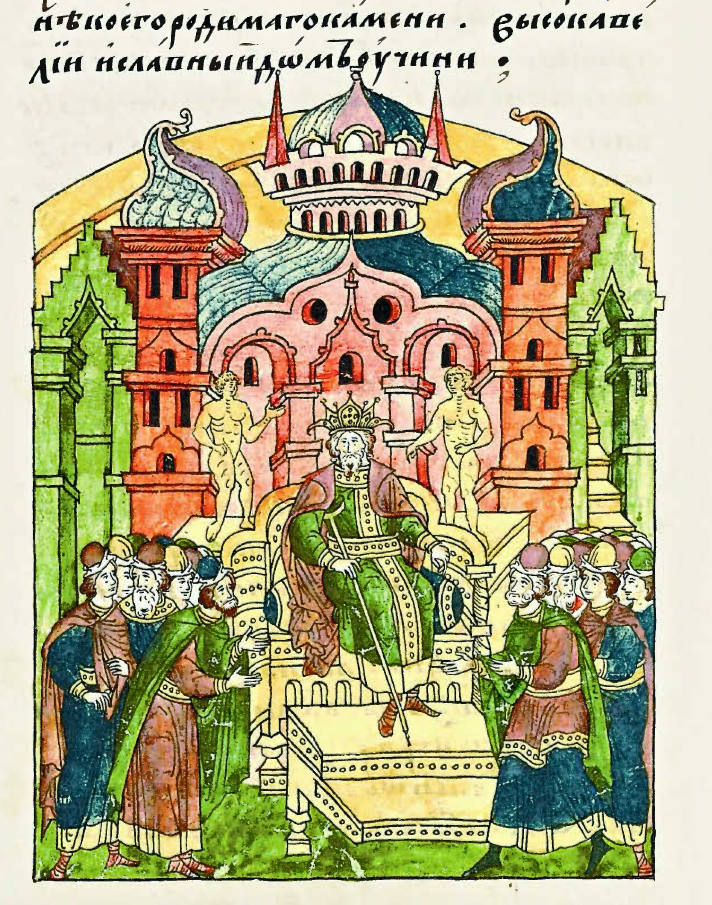
\includegraphics[width=\linewidth]{chast-troya/drugie/svod-01.jpg}

\textit{Иллюстрация к сему из Лицевого свода.}
\end{center}
\vspace*{\fill}
\newpage

А теперь – описание Илиона из Лицевого свода. Под Илионом подразумевается укрепленная область внутри самой Трои, на горе. В Илионе помещается царский дворец.

\begin{quotation}
Написание нарочитые Илионы:

Илион утвердитися устрои, яже его двор царсий полата нарицается и великия крепости на сем камени родственом силою отсечено утверждена бе славная Илион. 

Отнизу же иже горе круглым образом заключена, ея же высота 500 пасеус\footnote{Вероятно, под «пасеус» имеется в виду римская мера длины «pace», равная 1,48 метра.} досягаше. кроме верхов стрелничих окрест себе немногим разстоянием стоящих. иже много тоя высоту превосхожаху. коих стрелницы высоты ради, высоты зелные облачным одеянием. всегдашними излиянии покрывахуся и от их высоты толь велие и вся прилежащая в себя страны мста и далная паки град добре можаху видети.

Сея полаты стены, яже зрящим видяхуся не от мелнечныя извести светлая убеления светяху. зане все беша камени мраморными украшена. во многоцветном различии разделены и празднественых образов резании. яже зрящих образы веселяше. сице в окна их незнаменашеся дело некако мраморное. поне болшая часть их сооружена бе от четвероуголных блистаемых. клисталных. Тако тех вокон столпцы и забрала от внутрение страны предиреченные полаты. промеж иными здании каморными. чюдне царь Приям некую полаты постави. долготы великие. на широты равные. 

Ея же внешнее лице бе децками мраморными одеянно  и от древ кедровых и ливановых свод ея дощан. Ея же мост водовиднаго дела разноличным существом разными разделяше цветы.

В начале бе сия полаты и царьский престол поставлен. идеже стол царский и долгим величеством протягновен бе, весь составлен из слоновых изящных костей сице ото обою страну столов чин простерт. угодные даваше возлежащим седаниа.

В другом убо угле полаты тоя чюднаго дела бисеры и златом сотвореннаго некий создан олтарь бе во имя Зевса. К нему же дватцатию степенеи водовиднаго дела учинением блистателные приходящим безъструдный давашеся восход.

Наверху сего олтаря блисташеся прямо поставленый образ некии злат бога Зевся в долготу 15 лакот, весь от злата избранна составлен в непщевании великия цены. Его же разных бисеров украшаше напечатание и его существо благочествоваху злата отвсюду обложеннаго в разных делех соединения.

Сего бога Зевся образ бе Прияма царя наивышшее и непоколебимое упование, зане мняше тем в долгом благочестии царства его пребыти престолу и скипетра его власти в безконечные в веки предложити.

По сем же, егда царь Приям по непщеванию мысли своея Трою град преумыслимым концем сверши, внятным сердцем разгада вся и прилежною мыслию разъсмотрев град, от себе созданный, и толику крепостию цвести в силе крепости и твердости и толикими людми наполнен.
\end{quotation}

И видите – как отличается «гомеровская» Троя от той, что описана в русских источниках? У Гомера – Троянская равнина, на ней город Троя или Илион, а по равнине вне города – две реки, Ксанф-Скамандр и Симоент. Русская Троя – город, по нему, по середине его, течет Ксанктум, а на горе есть отдельная крепость Илион (Илиум), там же царский дворец. Река Симоент – в русских источниках – морской залив Семионт.

Откроем теперь старославянский перевод «Хроники Иоанна Малалы», который Истрин печатал по частям в 19 веке, да вышло еще издание в 1994-м\cite{malala01}. Перевод замечательный многими вещами – их надо тщательно изучать и делать открытия, но сие выходит на рамки этой книги. Например, имена некоторых греческих богов заменены славянским – Дый, Сварог, Дажбог. 

Пятая книга, про Трою, озаглавлена «Книгы завета бжия ветха сказающе образы новаго завета истиннно соуще преложеныя с греска языка в словенскый...» – переводчик или сам Малала относил историю про Трою к набору священных христианских книг. Кажется, книжники Ивана Грозного были того же мнения, раз включили повесть о Трое в Лицевой свод следом за «библейскими» томами.

По хронике, сюжетно сходной с «Илиадой» и «Одиссеей», Троя лежит в стране Фругеистей. Ученые трактуют это слово как «Фригийской», от Фригии, давней стране в Малой Азии, западной части. Трою относят к Фригии и в некоторых других старинных источниках, в том числе скандинавских. Однако, между Фригией и Троадой лежала Мисия.

Уместно вспомнить старинное русское слово «фряг», которым обозначали то немцев, то французов, то вообще иностранцев. Его сходство с «враг» и «варяг» очень настораживает. А в Варяжской пещере так и слышится – Фряжская пещера. Это о сходстве слов!

Троя в Хронике называется так: Или град, Илии град. Также: Труа, Труя, град Илии и Дардане. Приам именуется царем Фругийским и Асийским. А Труя и Илиа были царями, сыновьями царя Дана. Многократно упоминаются то как два отдельных града Илиа град и Троя град, то, кажется, взаимозаменяемые имена одного града.

Действующие лица сюжета о Троянской войне описаны порой с той же удивительной подробностью, что отличает «Илиаду». Будто в хронику из отдельного источника вносятся сохраненные кем-то описания: «Патроклос толст, силен, середнии, добролик, доброок нароус, чист, румян, добробрад, блгороден, храбор, крепок». «Ектор смагл, высок, зело благ, и силен крепостию, добронос, кудряв, коротовлас, добробрад, прилепном языком, благороден, и горд, храбор, тяжкогласен». И так несколько страниц!

На подробности о самой Трое хроника скупа. Есть про реку Ксандр, куда Эллины загнали противника «и побегшим впадаша многы в Ксандр и истопоша».

Поскольку хроника Малалы – сведение из разных источников, Малала, где может, называет их, например:

\begin{quotation}
си же Сисоуфос Койскыи спис, в вои сам быв с Теоукром, иже списание обрете Омир Илиаду списа и Виргилиус другое. еже в рапсодии Сисуфа пишется, еже писано, по многе летех Омира и Виргилиа обретены бы при Клавдии Нероне цри.
\end{quotation}

Здесь Малала говорит, что эту историю описал Сисоуфос Койской, который вместе с Теоукром участвовал в Троянской войне. И мол, это же описание обрели Гомер (Омир), написав «Илиаду», и Виргилий. И как сказано в расподии Сисуфа, писания Омира и Виргилия спустя многие годы стали известны при Клавдии Нероне\footnote{Вероятно, речь идет об известнейшем из Неронов, потому что их было несколько.}.

Сколько же было этих описаний, переложений, переводов, пересказов? Что осталось в них истинного, кроме названия Трои? 

Как именно могло изменяться повествование о Трое? Вот есть Фрэнка Баума «Волшебник из Страны Оз». А наш Волков ее пересказал и получился «Волшебник Изумрудного города». В литературе и кино не редкость перенос сюжета из одной среды в другую, из одного времени и страны в другие.
